\documentclass{article}
\usepackage[left=1.8cm,right=3cm,top=2cm,bottom=2cm]{geometry} % page
% settings
\usepackage{multicol} 
\usepackage{amsmath} % provides many mathematical environments & tools
\usepackage{dsfont}
\usepackage{upgreek}
\usepackage[spanish]{babel}
\usepackage[doument]{ragged2e}

% Images
\usepackage{graphicx}
\usepackage{float}
\usepackage{subfigure} % subfiguras
\usepackage{caption}
\captionsetup[table]{labelformat=empty}
\captionsetup[figure]{labelformat=empty}

% Code
\usepackage{tikz}
\usetikzlibrary{automata,positioning}
\usepackage{pgfplots}
\usepackage{color}

\usepackage{listings}
\usepackage{xcolor}
\definecolor{gray}{rgb}{0.5,0.5,0.5}
\newcommand{\n}[1]{{\color{gray}#1}}
\lstset{numbers=left,numberstyle=\small\color{gray}}

\selectlanguage{spanish}
\usepackage[utf8]{inputenc}
\setlength{\parindent}{0mm}

\begin{document}

\title{Trabajo 1: Programación}
\author{Patricia Córdoba Hidalgo}
\date{}
\maketitle

\tableofcontents

\section{EJERCICIO SOBRE LA COMPLEJIDAD DE H Y EL RUIDO}

Este ejercicio está implementado en el fichero \texttt{ejercicio1.py}.\\

\subsection{Apartado 1}

Se generaron las dos siguientes nubes de puntos diferentes a partir de una muestra de tamaño 50.

\begin{figure}[H]
  \centering
  \subfigure[Nube generada uniformemente]{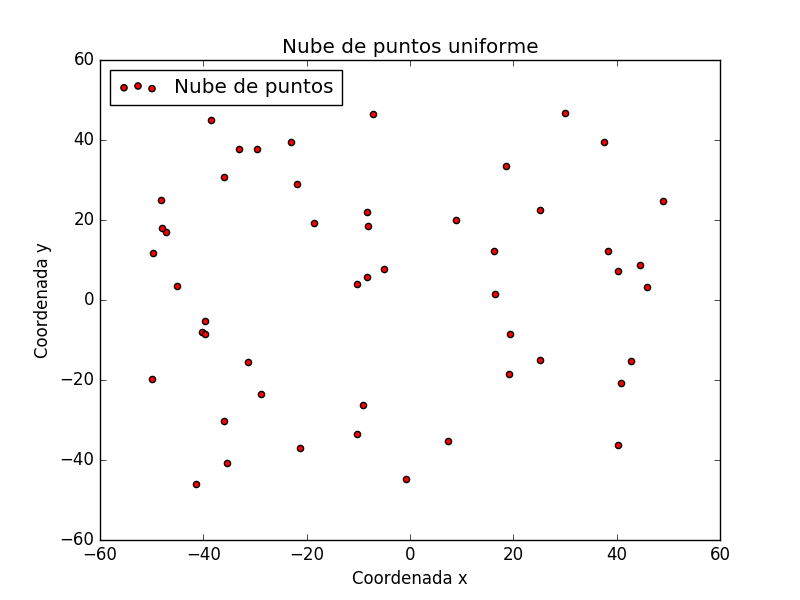
\includegraphics[width=83mm]{imgs/nube_unif_50}}
  \subfigure[Nube generada con una distribución Gaussiana]{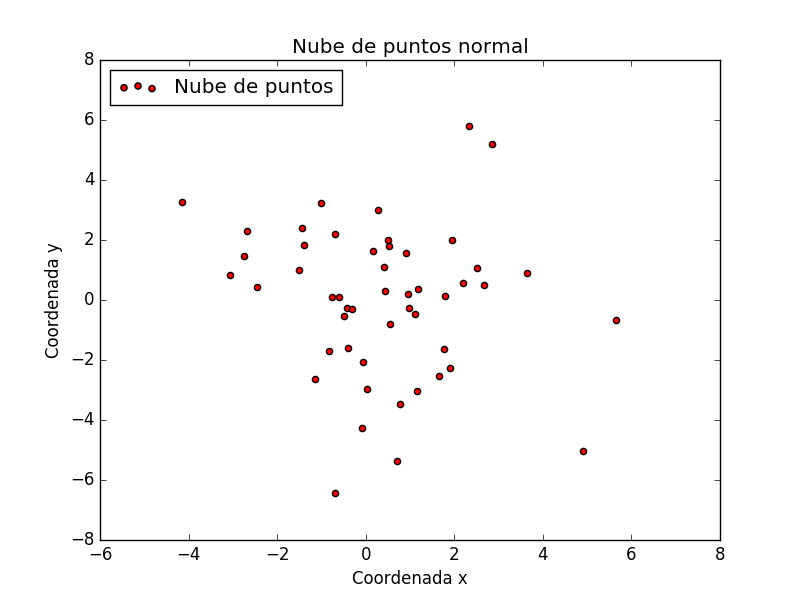
\includegraphics[width=83mm]{imgs/nube_normal}}
\end{figure}

La primera se generó usando la función \texttt{simula\_unif} y la segunda con la función \texttt{simula\_gaus}, ambas nos las daban ya implementadas. Tras esto, se usa la función \texttt{muestra\_datos} que representa los puntos de ambas nubes.

\subsection{Apartado 2}

Etiquetamos una muestra de 100 puntos escogidos uniformemente en el cuadrado $[-50, 50] \times [-50, 50]$ según el signo de la función $f(x,y) = y + 2.45627963467703x - 116.24116219196964$, usando \texttt{simula\_recta} para generar la recta y \texttt{asigno\_etiquetas} para etiquetar los datos. La gráfica de los puntos con su etiqueta correspondiente es:

\begin{figure}[H]
  \centering
  \subfigure[Datos sin ruido]{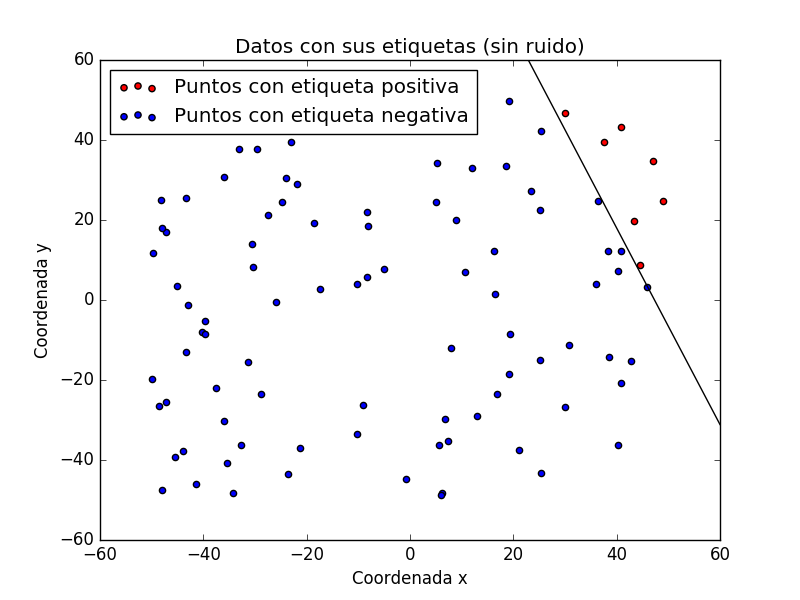
\includegraphics[width=110mm]{imgs/datos_sin_ruido}}
\end{figure}

Modifiqué el 10\% (aproximadamente, ya que trunco a la baja) de las etiquetas de los datos con la función \texttt{asigna\_etiquetas\_ruido}. La gráfica con los datos nuevamente etiquetados es:

\begin{figure}[H]
  \centering
  \subfigure[Datos con ruido]{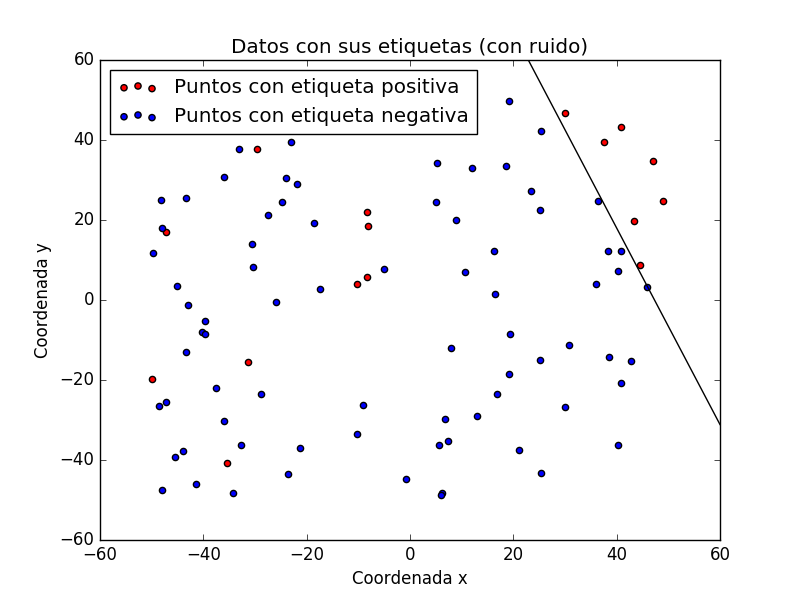
\includegraphics[width=100mm]{imgs/datos_con_ruido}}
\end{figure}

Tras esto, se usaron cuatro clasificadores diferentes sobre los datos etiquetados, ya que, al añadir ruido, pudiera ser que alguno de estos clasificadores de orden cuadrático cometiese un menor error que la recta que se usó para asignar las etiquetas originalmente, que ahora produce un error del 10\%. Las gráficas con esos clasificadores son:

\begin{figure}[H]
  \centering
  \subfigure[$f1(x,y) = (x-10)^2+(y-20)^2-400$]{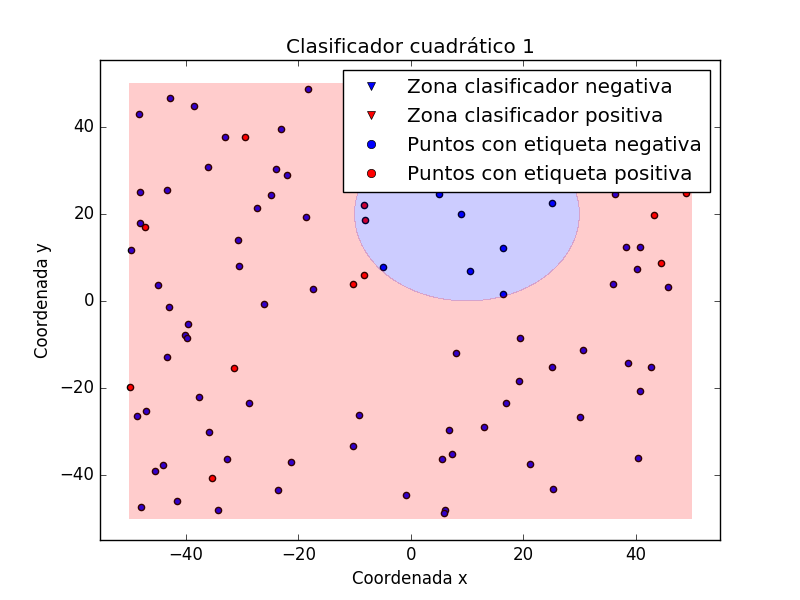
\includegraphics[width=83mm]{imgs/cla1}}
  \subfigure[$f2(x,y) = 0.5(x+10)^2+(y-20)^2-400$]{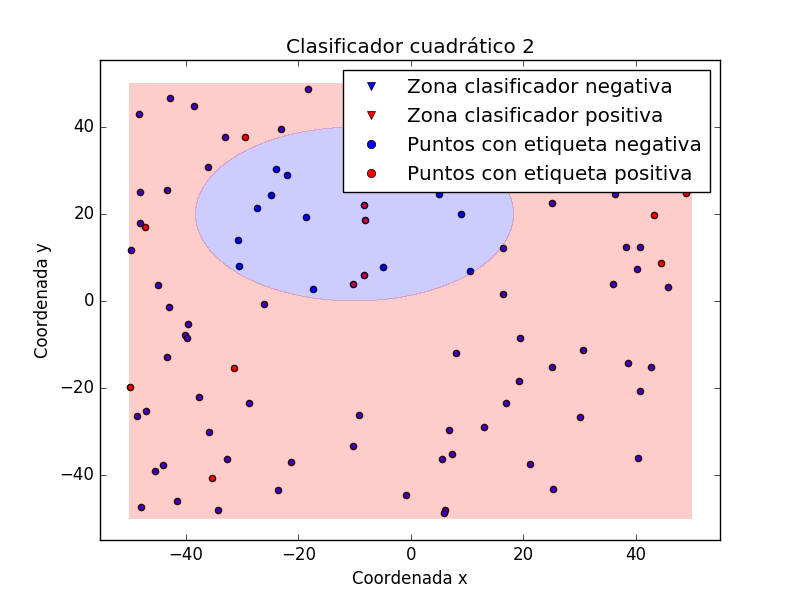
\includegraphics[width=83mm]{imgs/cla2}}
  \subfigure[$f3(x,y) = 0.5(x-10)^2-(y+20)^2-400$]{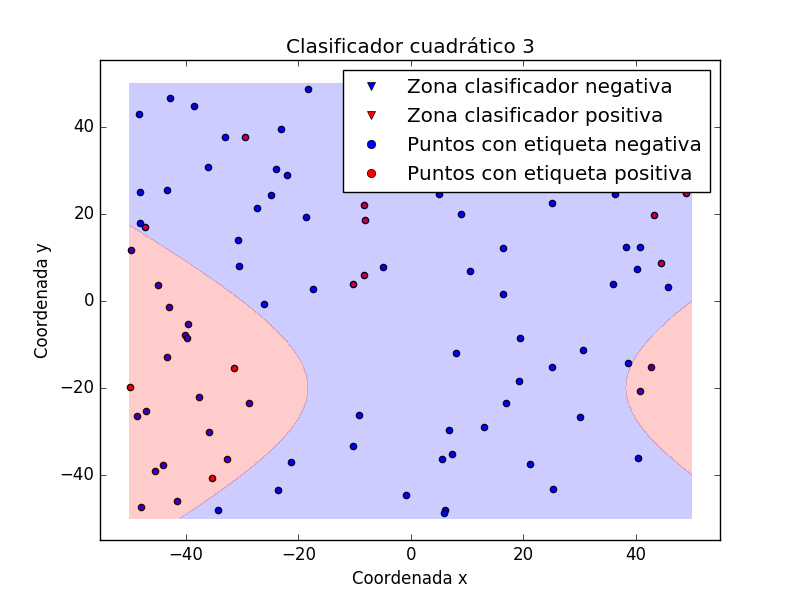
\includegraphics[width=83mm]{imgs/cla3}}
  \subfigure[$f4(x,y) = y-20x^2-5x+3$]{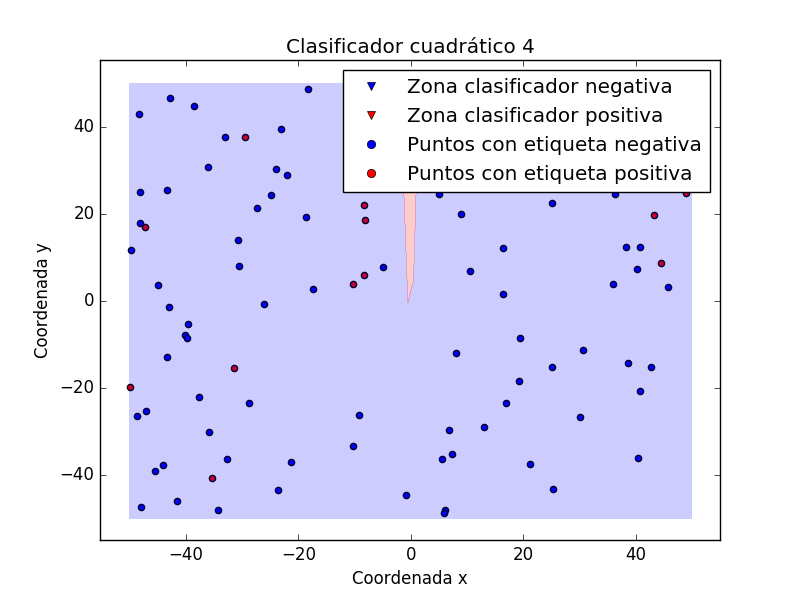
\includegraphics[width=83mm]{imgs/cla4}}
\end{figure}

Estas graficas se representaron con la función \texttt{graficaf}.
Usando como función de error el porcentaje de datos mal clasificados, implementada en la función \texttt{Err}, el error de cada clasificador es:

\begin{center}
\begin{tabular}{|c|c|}
\hline
\multicolumn{1}{|c|}{\textbf{Función}}& 
\textbf{Error}  \\ \hline
  a) $(x-10)^2+(y-20)^2-400$    & 75\% \\
  b) $0.5(x+10)^2+(y-20)^2-400$ & 75\% \\
  c) $0.5(x-10)^2-(y+20)^2-400$ & 32\% \\
  d) $y-20x^2-5x+3$             & 16\% \\ \hline
\end{tabular}
\end{center}

Por tanto todos estos clasificadores tienen mayor error que la recta original, luego son peores que la función lineal.\\

En el proceso de aprendizaje, al extraer datos con sus etiquetas siempre estamos expuestos a que las etiquetas tengan un error respecto a la función real que las etiquetó. Es por esto que a veces, aunque la función real que etiqueta es una función lineal, por el comportamiento de los datos de la muestra, podríamos encontrar una función más compleja con menor error muestral. Con esto podemos producir sobreajuste, ya que intentar buscar funciones complejas que minimicen el error en la muestra puede acarrear un aumento del error $E_{out}$, ya que las clases de funciones complejas tienen una mayor varianza y con muestras muy pequeñas el error $E_{out}$ varía mucho del $E_{in}$.\\
En nuestro caso específico, podemos ver que las funciones más complejas elegidas tienen mayor $E_{in}$ que la  original, luego no hay duda de que ésta es la mejor función encontrada para clasificar esta muestra.

\section{MODELOS LINEALES}

\subsection{Algoritmo Perceptron}

Programé la función \texttt{ajusta\_PLA} para calcular el hiperplano solución al problema de clasificación. En mi caso, la entrada \textit{datos} es una matriz donde cada fila es un item de la forma $x = [1 \hspace{3mm} coordenada\hspace{1mm}X \hspace{3mm} coordenada\hspace{1mm}Y]$, ya que meter las etiquetas en la matriz era redundante e innecesario al tener el vector de etiquetas \textit{label}.\\

Ejecutamos el \textit{Algoritmo del PLA} con la muestra del apartado  2 usando etiquetas sin ruido. Las gráficas obtenidas (en el caso del vector aleatorio con el último de los 10 usados) son:

\begin{figure}[H]
  \centering
  \subfigure[Vector inicial cero]{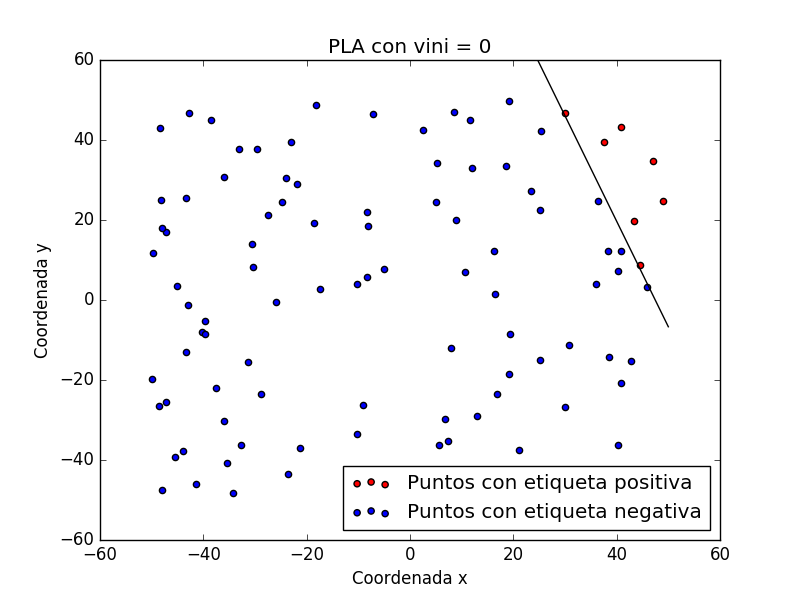
\includegraphics[width=83mm]{imgs/PLA_sin_ruido_0}}
  \subfigure[Vector inicial aleatorio]{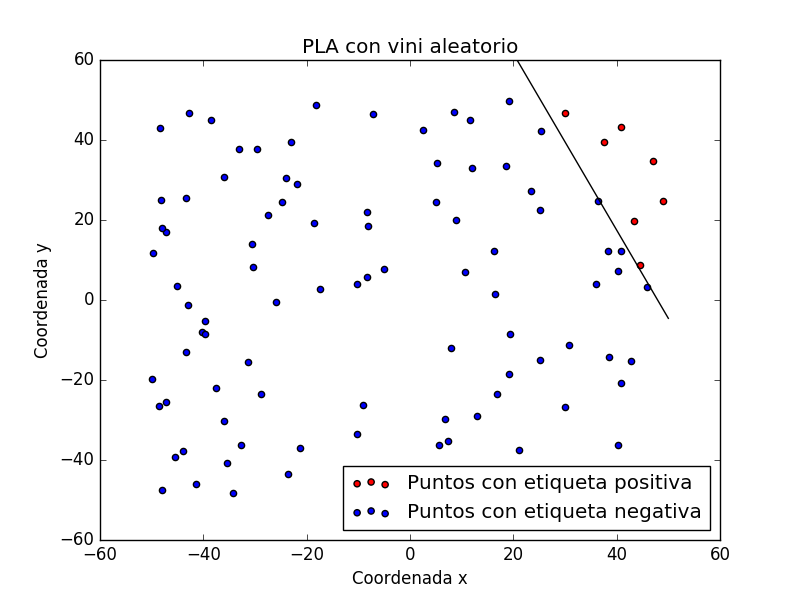
\includegraphics[width=83mm]{imgs/PLA_sin_ruido_alea}}
\end{figure}

Usando como vector inicial el vector cero, el algoritmo converge en 444 iteraciones, obteniendo los pesos $w = [ -2129 \hspace{3mm} 44.85508745 \hspace{3mm} 17.01070298 ]$. Usando 10 vectores iniciales aleatorios, la media es de 17 iteraciones, y en la última iteración los pesos obtenidos son $w = [ -412.45365318 \hspace{3mm} 8.60651887 \hspace{3mm} 3.90172468]$. Como podemos observar, en mi caso el punto inicial influye bastante en el número de iteraciones.\\

Ejecutando el \textit{Algoritmo del PLA} con la muestra del apartado  2 usando etiquetas con ruido obtenemos las siguientes gráficas:

\begin{figure}[H]
  \centering
  \subfigure[Vector inicial cero]{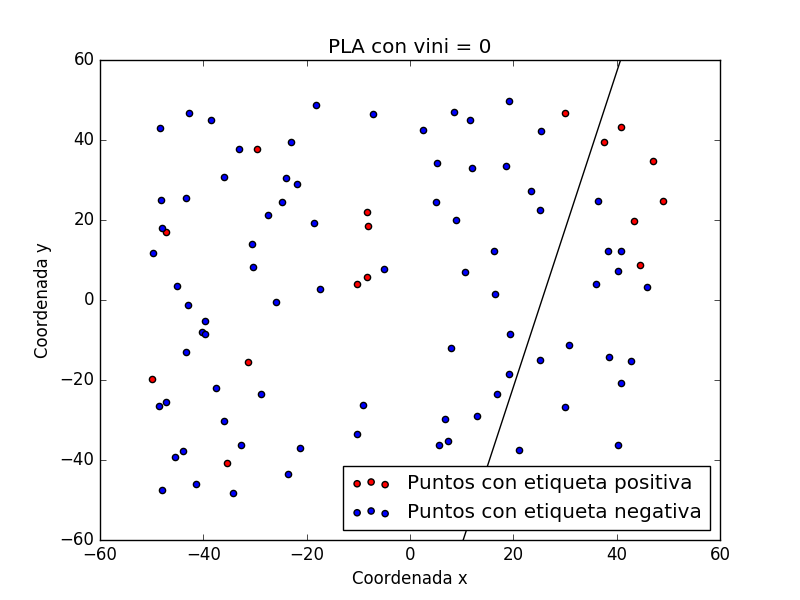
\includegraphics[width=83mm]{imgs/PLA_ruido_0}}
  \subfigure[Vector inicial aleatorio]{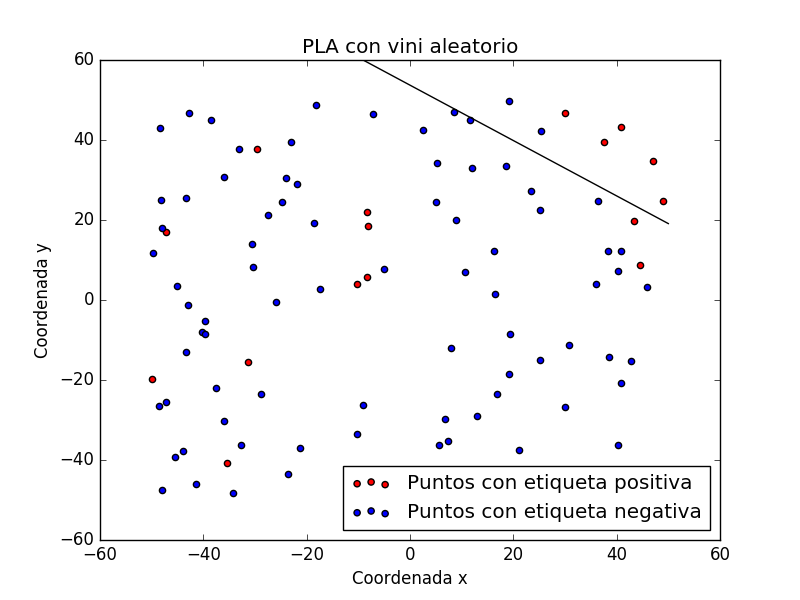
\includegraphics[width=83mm]{imgs/PLA_ruido_alea}}
\end{figure}

En este caso los conjuntos no son separables, por lo que el \textit{Algoritmo del PLA} no converge nunca. Por tanto, éste ciclará indefinidamente y devolverá el resultado de la última ejecución realizada, que no tiene por qué ser el resultado con menor error de todos los obtenidos en las diferentes iteraciones. 

\subsection{Regresión Logística}

Usando la función \texttt{simula\_unif} creamos una muestra de 100 puntos uniformemente distribuidos en el cuadrado $[0,2] \times [0,2]$ ycon la función \texttt{simula\_recta} seleccionamos la línea del plano que será la frontera de la función $f(x)$. Se asignan etiquetas a los puntos del cuadrado con \texttt{asigno\_etiquetas}, dandole a los puntos por encima de la recta, que son aquellos con $f(x)=1$ la etiqueta $y=1$ y a los de debajo de la recta, que son aquellos con $f(x)=0$, etiqueta $y=-1$.

Se implementó el algoritmo de \textit{Regresión Lineal} obteniendo el siguiente resultado:

\begin{figure}[H]
  \centering
  \subfigure[Regresion Logística]{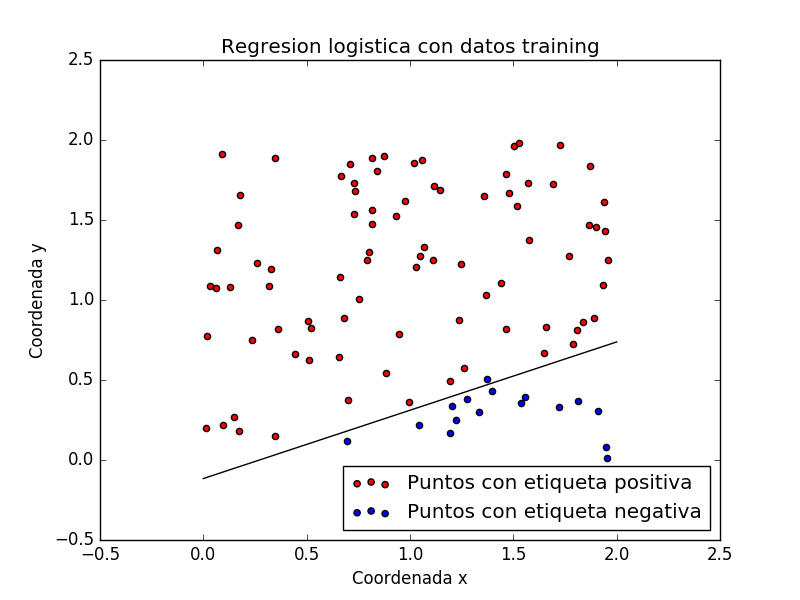
\includegraphics[width=83mm]{imgs/rl}}
\end{figure}

La función obtenida con el algoritmo es $g(x)= \frac{1}{1}$, donde $w = [0.6206406 \hspace{3mm} -0.94098291 \hspace{3mm} 2.57813861]$.

El error $E_{out} = 0.22651876695632325$ y el $E_{in} = 0.20481405394280924$.

\section{BONUS}

El problema es clasificar un conjunto de dígitos en dos clases diferentes, los cuatros y los ochos.
El modelo usado es el siguiente:\\
Los datos son de la forma $x_i = (1, x1, x2)$, donde $x1$ es la intensidad promedio y $x2$ es la simetría. Las etiquetas correspondientes son $y_i \in \{1, -1\}$. Inicialmente $y_i = 1$ si $x_i = 8$ y $y_i = -1$ si $x_i = 4$.
Usando el algoritmo de \textit{Gradiente Descendente Estocástico} y \textit{Matriz Pseudoinversa} se obtiene $w$, que son los pesos de la función $h$ que aproxima a la función $f$ desconocida que a cada $x$ le asigna su etiqueta correspondiente. Tenemos pues que $h(x_i) = w_0 + w_1x1 + w_2x2$, con $w = (w_0, w_1, w_2)$.\\


\end{document}
